\documentclass{article}
\usepackage[utf8]{inputenc}
\usepackage[spanish,mexico]{babel}
\usepackage[margin=2.3cm]{geometry}
\usepackage{graphicx}
\usepackage[export]{adjustbox}
\usepackage{caption}
\usepackage{subcaption}
\usepackage{fancyhdr}
\usepackage{lipsum}
\usepackage{float}
\usepackage{enumerate}
\usepackage{array}
\usepackage{float}

% >
\usepackage{ tipa }

%\usepackage{multirow}
\usepackage[spanish,es-tabla]{babel}

% Comentario en varias líneas
\usepackage{comment}

% Importar código de algún lenguaje
%\usepackage{listings}
%\lstset{
%  language=Scheme
%}
\usepackage{xcolor}

\definecolor{codegreen}{rgb}{0,0.6,0}
\definecolor{codegray}{rgb}{0.5,0.5,0.5}
\definecolor{codepurple}{rgb}{0.58,0,0.82}
\definecolor{backcolour}{rgb}{0.95,0.95,0.92}

%\lstdefinestyle{mystyle}{
%    backgroundcolor=\color{backcolour},
%    commentstyle=\color{codegreen},
%    keywordstyle=\color{magenta},
%    numberstyle=\tiny\color{codegray},
%    stringstyle=\color{codepurple},
%    basicstyle=\ttfamily\footnotesize,
%    breakatwhitespace=false,
%    breaklines=true,
%    captionpos=b,
%    keepspaces=true,
%    numbers=left,
%    numbersep=5pt,
%    showspaces=false,
%    showstringspaces=false,
%    showtabs=false,
%    tabsize=2
%}

%\lstset{style=mystyle}

% Evitar sangrías
\setlength{\parindent}{0cm}

% Formato para estructuras como with.
\usepackage{listings}

% Código
\newcommand{\code}[1]{\textcolor{white!25!black}{\texttt{#1}}}

% Letter colors.
\usepackage{xcolor}

% Columnas multiples
\usepackage{multicol}

\usepackage{amsmath}
%%\usepackage{graphicx}
%%\usepackage{subcaption}
\usepackage{amsmath}
\usepackage{amssymb}
\usepackage{amsthm}
\usepackage{url}

%%Tablas con color
\usepackage{xcolor, colortbl}
\usepackage{array, multirow, multicol}
\cellcolor[modelo color]{color}

\pagestyle{fancy}
\fancyhf{}

\title{Facultad de Ciencias, UNAM}
\date{\today}

\begin{document}

\thispagestyle{empty}

	\begin{figure}[ht]
	   \minipage{0.76\textwidth}
			
\includegraphics[width=4cm]{Logo_UNAM.png}
			\label{EscudoUNAM}
	   \endminipage
	   \minipage{0.32\textwidth}
			
\includegraphics[height = 4.9cm ,width=4cm]{Logo_FC.png}
			\label{EscudoFC}
		\endminipage
	\end{figure}

	\begin{center}
	\vspace{0.8cm}
	\LARGE
	UNIVERSIDAD NACIONAL AUTÓNOMA DE MÉXICO

	\vspace{0.7cm}
	\LARGE
	FACULTAD DE CIENCIAS

	\vspace{0.8 cm}
	\Large
	\textbf{Tarea 6}

	\vspace{0.8 cm}
	\normalsize
	INTEGRANTES \\
	\vspace{.2cm}
	\large
	\textbf{Torres Valencia Kevin Jair - \texttt{318331818}}\\
	\textbf{Aguilera Moreno Adrián - \texttt{421005200}}\\
	\textbf{Rivera Silva Marco Antonio - \texttt{318183583}}\\
	%\textbf{Nombre - \texttt{Número de cuenta}}

	\vspace{1 cm}
	\normalsize
	PROFESORA \\
	\vspace{.2cm}
	\large
	\textbf{Karla Ramírez Pulido}

	\vspace{1 cm}
	AYUDANTES \\
	\vspace{.2cm}
	\large
	\textbf{Alan Alexis Martínez López}\\
	\textbf{Manuel Ignacio Castillo López}\\
	\textbf{Alejandra Cervera Taboada}
	\vspace{1.3cm}

	\normalsize
	ASIGNATURA \\
	\vspace{.2cm}
	\large
	\textbf{Lenguajes de Programación}

	\vspace{1 cm}
	\today
	\end{center}

	\newpage
	\textbf{\textcolor{blue}{1.}} \Large
Currifica cada uno de los siguientes términos.

\renewcommand{\theenumi}{\alph{enumi}}
\begin{itemize}

\item $\lambda abc.abc$.\\
\textbf{Solución:}
$\lambda a. \lambda b. \lambda c. abc$
%%%%%%%%%%%%%%%%%%%%%%%%%%%%%%%%%%%%%%%%%%%%%%
\item $\lambda abc. \lambda cde.acbdce$.\\
\textbf{Solución:}
$\lambda a.\lambda b.\lambda c.\lambda c.\lambda d.\lambda e.acbdce$
%%%%%%%%%%%%%%%%%%%%%%%%%%%%%%%%%%%%%%%%%%%%%%
\item $(\lambda d.(\lambda de.e) (\lambda fc.c)) (\lambda ab.b)$.\\
\textbf{Solución:}
$(\lambda d.(\lambda d.\lambda e.e)(\lambda f.\lambda c.c))(\lambda a.\lambda b.b)$
\end{itemize}

	\textbf{\textcolor{blue}{2.}} \Large
Aplica $\alpha$-conversiones en cada expresión
para cambiar los términos de las variables de ligado.
\begin{enumerate}[a)]
%%%%%%%%%%%%%%%%%%%%%%%%      Inciso a    %%%%%%%%%%%%%%%%%%%%%%%%%%%%
    \item $\lambda a.\lambda b.(\lambda a.b \; \lambda b.a)$
%%%%%%%%%%%%%%%%%%%%%%%%      Inciso b    %%%%%%%%%%%%%%%%%%%%%%%%%%%%
    \item $\lambda a.(a(\lambda b.(\lambda a.a\; b)a))$
%%%%%%%%%%%%%%%%%%%%%%%%      Inciso c    %%%%%%%%%%%%%%%%%%%%%%%%%%%%
    \item $\lambda x.(\lambda y.x\; \lambda y(\lambda x.x \; y))$
\end{enumerate}

	\textbf{\textcolor{blue}{3.}} \Large
Aplica $\beta$-reducciones a las siguientes expresiones
para llegar a una Forma Normal, en caso de que no se pueda justifica. Además indica
en cada paso el reducto y el redex.\\

$l\;=_{def} \lambda a.a$\\
$K\;=_{def} \lambda a.\lambda b.a$\\
$S\;=_{def} \lambda a.\lambda b.\lambda a.ac(bc)$\\
$\Omega\; =_{def} (\lambda a.aa) (\lambda a.aa)$

\begin{enumerate}[a)]
%%%%%%%%%%%%%%%%%%%%%%%%      Inciso a    %%%%%%%%%%%%%%%%%%%%%%%%%%%%
    \item $\lambda a.aK\Omega$

    \textbf{Solución:}
    \begin{eqnarray*}
        \lambda_a .aK\Omega &\equiv& \lambda_a .a
        (\lambda_a . \lambda_b . a)
        ((\underbrace{\lambda a.aa}_{Redex}) (\lambda a.aa))\\
        &\rightarrow_{\beta}&
        \lambda_a .a (\lambda_a .a)(\underbrace{(\lambda a.aa) (\lambda a.aa)}_{Reducto}).
    \end{eqnarray*}
    Esta $\lambda$-función diverge, como se puede observar en la $\beta$-reducción anterior.
%%%%%%%%%%%%%%%%%%%%%%%%      Inciso b    %%%%%%%%%%%%%%%%%%%%%%%%%%%%
    \item $(\lambda a.a(ll))c$

    \textbf{Solución:}
    \begin{eqnarray*}
        (\lambda_a .a(ll))c &\equiv& \lambda_a . a((\underbrace{\lambda_a .a}_{Redex})
        (\lambda_a .a))c\\
        &\rightarrow_{\beta}& \lambda_a .
        a(\underbrace{\lambda_a .a}_{\text{Reducto y Redex}})c\\
        &\rightarrow_{\beta}& \underbrace{\lambda_a . a}_{Redex} \underbrace{c}_{Reducto}\\
        &\rightarrow_{\beta}& \underbrace{c}_{Reducto}.
    \end{eqnarray*}
%%%%%%%%%%%%%%%%%%%%%%%%      Inciso c    %%%%%%%%%%%%%%%%%%%%%%%%%%%%
    \item $(\lambda d.\lambda e.(\lambda f.f(\lambda a.ad))e)b(\lambda c.\lambda b.cb)$

    \textbf{Solución:}
    \begin{eqnarray*}
        (\lambda_d .\lambda_e .(\underbrace{\lambda_f .f}_{Redex}
        (\lambda_a .ad))e)b(\lambda_c .\lambda_b .cb)
        &\rightarrow_\beta&
        (\lambda_d .\lambda_e
        .(\underbrace{\overbrace{\lambda_a .a}^{Redex}d}_{Reducto})e)
        b(\lambda_c .\lambda_b .cb)\\
        &\rightarrow_\beta& (\lambda_d .\overbrace{\lambda_e .\underbrace{e}_{Reducto}}^{Redex}
        (d) b(\lambda_c .\lambda_b .cb)\\
        &\rightarrow_\beta& (\overbrace{\lambda_d .\underbrace{d}_{Reducto}}^{Redex}
        (b)(\lambda_c .\lambda_b .cb)\\
        &\rightarrow_\beta& \underbrace{b}_{Reducto}
        ((\underbrace{\lambda_c .\lambda_b .c}_{Redex})b)\\
        &\rightarrow_\beta& b \underbrace{\lambda_b . b}_{Reducto}.
    \end{eqnarray*}
\end{enumerate}

	\textbf{\textcolor{blue}{4.}} \Large
Usando recursión de cola optimiza la función del Ejercicio 2. Toda función auxiliar ocupada
debe ser optimizada.\\

	\Large\textbf{\textcolor{blue}{5.  *Punto extra*}} 
Observa la siguiente función del lenguaje de programación \code{Racket}

\begin{lstlisting}
(let ([sum (lambda (n) (if (zero? n) 0 (+ n (sum (sub1 n))))))])
      (sum 5))
\end{lstlisting}

\begin{enumerate}[a.]
%%%%%%%%%%%%%%%%%%%%%%%%%%%%%      Inciso A        %%%%%%%%%%%%%%%%%%%%%%%%%%%%%%%%%
\item Prueba la expresión en el intérprete de \code{Racket} y con base en la respuesta 
obtenida, explica el proceso que siguió el intérprete para llegar a ésta. Anexa una 
captura de pantalla del intérprete de \code{Racket} al probar la expresión.

\begin{figure}[h]
  \centering
  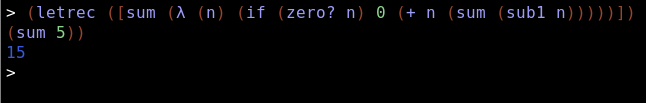
\includegraphics[scale=0.5]{./Sum.png}
  \caption{Ejecución de la función dada.}
\end{figure}

\begin{lstlisting}
> (let ([sum (lambda (n) (if (zero? n) 0 (+ n (sum (sub1 n))))))])
      (sum 5))
= (+ 5 (sum 4))
= (+ 5 (+ 4 (sum 3)))
= (+ 5 (+ 4 (+ 3 (sum 2))))
= (+ 5 (+ 4 (+ 3 (+ 2 (sum 1)))))
= (+ 5 (+ 4 (+ 3 (+ 2 (+ 1 0)))))
= (+ 5 (+ 4 (+ 3 (+ 2 (1)))))
= (+ 5 (+ 4 (+ 3 (3))))
= (+ 5 (+ 4 (+ 6)))
= (+ 5 (10))
= 15
\end{lstlisting}
%%%%%%%%%%%%%%%%%%%%%%%%%%%%%      Inciso B        %%%%%%%%%%%%%%%%%%%%%%%%%%%%%%%%%
\item Modifica la función usando el Combinador de Punto Fijo Y .Prueba la expresión en 
el intérprete de \code{Racket} y con base en la respuesta obtenida, explica el proceso que 
siguió el intérprete para llegar a ésta. Anexa una captura de pantalla del intérprete 
de \code{Racket} al probar la expresión.

\begin{figure}[h]
  \centering
  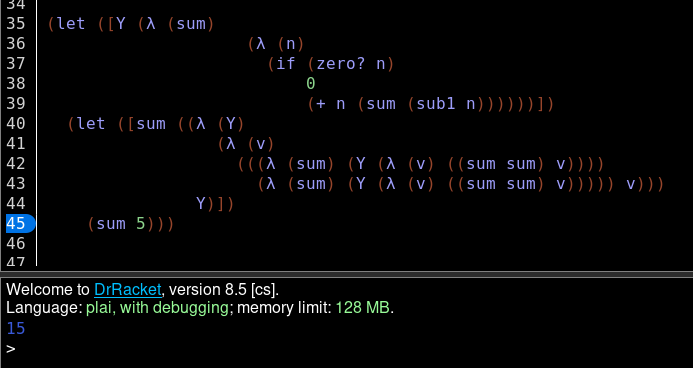
\includegraphics[scale=0.3]{./Sum-Y.png}
  \caption{Ejecución de la función dada.}
\end{figure}

Para esta función, tenemos una definición interna que realiza una recursión mutua,
la ejecución tiene que reducir las lambdas a su forma normal (en este caso siempre
es un valor numérico) y luego pasarselas a la función anterior o siguiente en el orden.
\newpage
%%%%%%%%%%%%%%%%%%%%%%%%%%%%%      Inciso C        %%%%%%%%%%%%%%%%%%%%%%%%%%%%%%%%%
\item Modifica la función usando el Combinador de Punto Fijo Z. Prueba la expresión en 
el intérprete de \code{Racket} y con base en la respuesta obtenida, explica el proceso que 
siguió el intérprete para llegar a ésta. Anexa una captura de pantalla del intérprete 
de \code{Racket} al probar la expresión.

\begin{figure}[h]
  \centering
  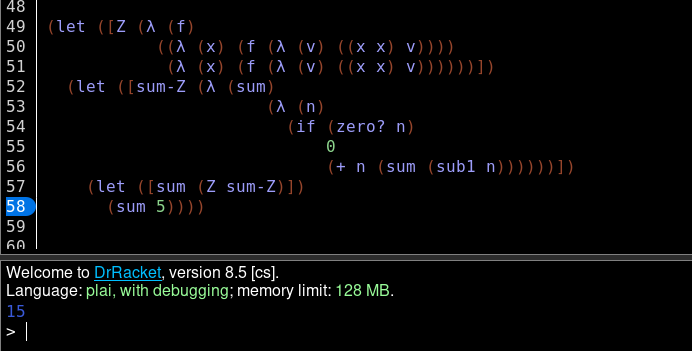
\includegraphics[scale=0.3]{./Sum-Z.png}
  \caption{Ejecución de la función dada.}
\end{figure}

Como en el ejercicio anterior, en la línea 27 se encuentra la modificación
que vuelve a esta función en un combinador de punto fijo Z. Inicialmente
reduce las lambdas a sus formas normales y ejecuta ambas funciones de manera
\textit{mutuamente recursiva} hasta llegar al valor deseado.
\end{enumerate}

\end{document}
